\documentclass{article}


\usepackage{arxiv}

\usepackage[utf8]{inputenc} % allow utf-8 input
\usepackage[T1]{fontenc}    % use 8-bit T1 fonts
\usepackage{hyperref}       % hyperlinks
\usepackage{url}            % simple URL typesetting
\usepackage{booktabs}       % professional-quality tables
\usepackage{amsfonts}       % blackboard math symbols
\usepackage{nicefrac}       % compact symbols for 1/2, etc.
\usepackage{microtype}      % microtypography
\usepackage{multicol}
\usepackage{lipsum}
\usepackage{graphicx}

\title{Classifying 2020 Presidential Candidate Speeches with Recurrent and Convolutional Neural Networks}


\author{
  Daniel Oshiro \\
  LIGN 167 \\
  University of California, San Diego\\
  \texttt{doshiro@ucsd.edu}
}

\begin{document}
\maketitle

\begin{abstract}
For the final project of LIGN 167, I built a recurrent neural network (RNN) using a gated recurrent unit (GRU) architecture and a convolutional neural network (CNN). I used these networks to classify presidential candidate speeches in the 2020 election. I built and trained the models in the PyTorch framework and found that the RNN had an accuracy of 47.347\% while the CNN had an accuracy of 33.311\%, significantly beating out the baseline model.
\end{abstract}

\section{Introduction}
With the rise of fake news and misinformation rapidly spreading through social media, it is important to be able to determine the truth of what one reads online. Further, with the upcoming 2020 election, it is important to understand each candidate's true positions and arguments. In order to solve this problem, I propose a neural network classifier that, given a part of a speech from a candidate, can determine who said it. To solve this problem, I proposed two network architectures, one RNN and one CNN to determine if either architecture excelled above the other. 

The rest of this paper is organized as follows: Section 2 defines the problem; Section 3 describes in depth the architecture and training of the RNN; Section 4 describes in depth the architecture and training of the CNN; Section 5 describes the results of the experiment; Section 6 concludes the paper, discussing potential improvements moving forward.

\section{Problem Definition}
Formally, the problem can be stated as the following:

Let $V$ be a set of words that form a vocabulary. Let $P \subset \mathbb{R}^{12}$ such that $|P| = 12$ and each $p \in P$ is a one-hot vector corresponding to one of the following candidates:
\begin{multicols}{3}
    \begin{enumerate}
        \item Michael Bennet
        \item Joseph Biden
        \item Cory Booker
        \item Pete Buttigieg
        \item Julián Castro
        \item John Delaney
        \item Kamala Harris
        \item Amy Klobuchar
        \item Bernie Sanders
        \item Donald Trump
        \item Elizabeth Warren
        \item Andrew Yang
    \end{enumerate}
\end{multicols}
Given a word sequence of length $N,$ $v = (v_1, v_2, \dots, v_N),$ the model needs to learn a function $f:v \to p$ such that $p \in P$ is the one-hot vector that corresponds to the candidate who said the words that comprise the sequence.

\subsection{Dataset}
The data used to train the models was collected from a variety of sources including interviews, op-eds, advertisements, and campaign speeches \cite{githubdataset}. After collection, the data set was cleaned by converting all words to lower case, adding spaces between tokens, and making each paragraph its own line. The result is a dataset comprised of a total of 4719 paragraphs. The breakdown of the data is shown in the table below.


\begin{table}[htb]
 \caption{Dataset Distribution}
  \centering
  \begin{tabular}{llll}
    \toprule
    \cmidrule(r){1-2}
    Name     & Training     & Testing    & Total  \\
    \midrule
    Bennet & 127  & 61    &  188 \\
    Biden  & 175  & 115     & 290\\
    Booker & 138  &  82 & 220\\
    Buttigieg & 657 & 337 & 994 \\
    Castro & 155 & 38 & 193\\
    Delaney & 182 & 53 & 235\\
    Harris & 200 & 92 & 292\\
    Klobuchar & 314 & 174 & 488\\
    Sanders & 294 & 59 & 353\\
    Trump & 303 & 88 & 391\\
    Warren & 297 & 157 & 454\\
    Yang & 387 & 233 & 620\\
    \bottomrule
  \end{tabular}
  \label{tab:table}
\end{table}

\section{Recurrent Neural Network Model}
I chose to implement an RNN as the first model for this task because it has shown promising results as a sequence classifier \cite{nnprimer} and it can take as input sequences of various lengths.

\subsection{Architecture}
Formally stated, the input of the RNN at each step $t_i$ is a hidden state, $(h_{i-1} \in \mathbb{R}^{30})$ and a word embedding $(w_i \in \mathbb{R}^{300})$ representing the next word in the paragraph. The output is the next hidden state $h_i.$ I used a GRU as my recurrent unit, as it avoids the vanishing gradient problem seen in classical RNNs and allows for longer connections between words (CITE). The GRU is implemented as having 2 layers and hidden dimension 30. For now, let the function being applied by the GRU simply be called GRU. The following subsection will discuss this in more detail.

\begin{equation}h_i = GRU(h_{i-1}, w_i)\end{equation}

 Thus, for a phrase of length $N$, $(v_1,v_2,\dots,v_N)$, we have that, setting $h_0 = 0,$ we can calculate the final hidden state $h_N$ through the repeated application of the recurrent unit. 
 
 The output of the network is calculated by applying a 2-layer perceptron with input $h_N$. The hidden layer of the MLP has dimension 100. The nonlinearity used is a ReLU. This, the MLP can be formally stated as follows
 
 \begin{equation}x' = W_2 ReLU(h_N W_1 + b_1) + b_2\end{equation}
 \begin{center} With $W_1 \in \mathbb{R}^{30 \times 100}, \; b_1 \in \mathbb{R}^{100}$ and $W_2 \in \mathbb{R}^{100 \times 12}, \; b_2 \in \mathbb{R}^{12}.$ \end{center}
 
 The output $(x' \in \mathbb{R}^{12})$ is run through a softmax function. The entry of the vector with the highest magnitude is then chosen as the network’s guess for which candidate said the inputted phrase. 


\begin{equation} x = p \in P \; | \; argmax(softmax(x'))= p. \end{equation}

Figure 1 shows the RNN architecture.

\begin{figure}[h]
\caption{RNN Archicture.}
\centering
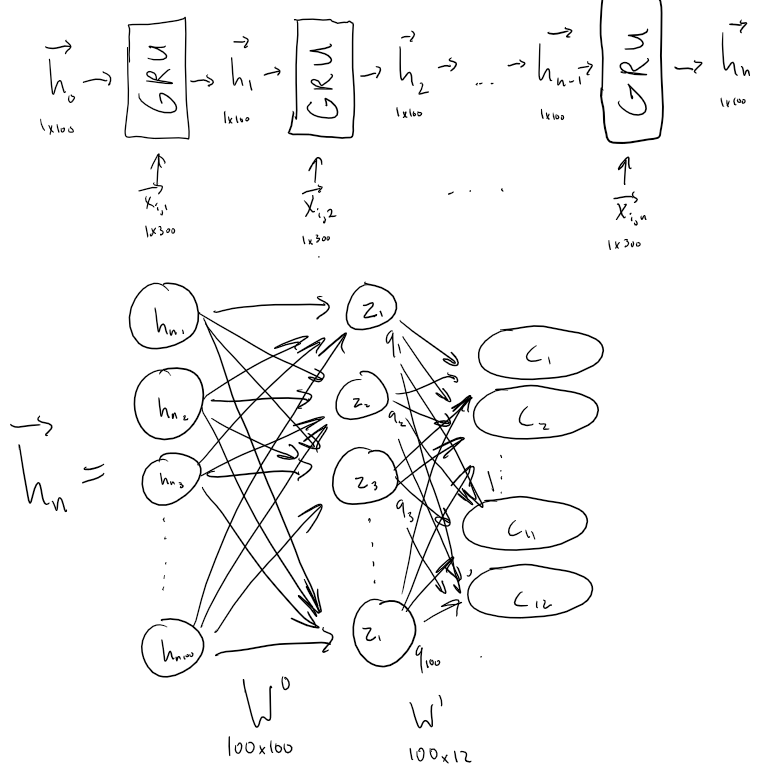
\includegraphics[width=0.5\textwidth]{RNN.png}
\end{figure}

\subsection{GRU Details}

Along with the hidden state $h_t$ off of which the MLP is trained, there are more hidden states in the GRU.
At each time step, we calculate a potential new hidden state $\tilde h_t.$ This value either replaces the current value of the hidden state or it doesn't, as determined by the relevance gates. The potential new hidden state can be calculated as follows. 
\begin{equation}\tilde{h_t} = \tanh(W \cdot [r_t * h_{t-1},x_t]).\end{equation}

The relevance gate $r_t$ determines the value of the previously calculated $\tilde h_t.$ The revelance gate is calculated as follows:

\begin{equation}r_t = \sigma(W_r \cdot[h_{t-1},x_t]).\end{equation}
The revelance gate uses the previous hidden state and the word inputted at the current time step to determine how relevant the current word is and determines whether or not to update the actual hidden state.

The GRU implementation diagram can be seen in figure 2.

\begin{figure}[h]
\caption{GRU Archicture from \cite{GRU}}
\centering
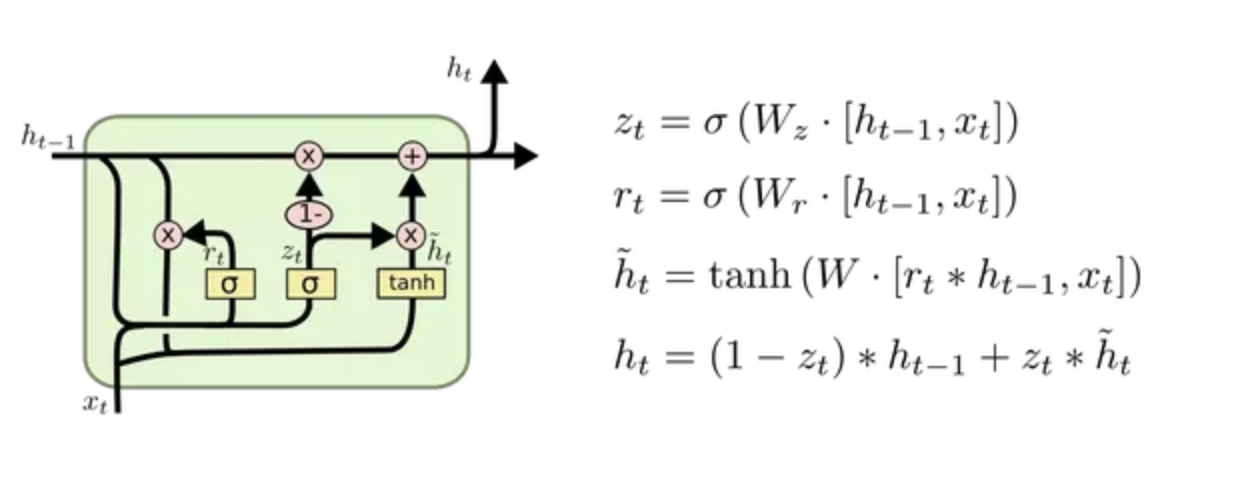
\includegraphics[width=0.5\textwidth]{GRU.png}
\end{figure}

\subsection{Training Details}
I implemented the model in PyTorch. The word embeddings are pre-trained GloVe embeddings of dimension 300. The hidden layer has dimension 30. The multilayer perceptron had a single, fully connected hidden layer of dimension 100. I used the Adam optimizer with learning rate $lr=0.001$. The model was trained with batch size of 256 over 100 epochs.


\section{Convolutional Neural Network Model}
I chose to implement a CNN because there is literature to suggest that a CNN can detect identifying features in text classification tasks due to a CNNs ability to identify key features associated with a particular class \cite{nnprimer}. 
\subsection{Architecture}
My implementation is modeled off of the CNN described here \cite{cnnpaper}. Again, I use GLoVe word embeddings of dimension 300. Padding is added to all the paragraphs so that they are the same length, in this case, each paragraph came out to $394$ words, with 0 padding added following the end of the paragraph. Thus, the paragraphs are inputs of $(w_1,w_2,\dots,w_{394})$ where $w_i \in W$ is a word embedding of dimension 300. Let $d$ be the depth of the convolutional layers. 

I computed each feature in the following manner. Let $h=3,4,5$ be the number of words over which we have the convolutional window. For each value of $i, \; 1\leq i \leq 394-h,$ I computed $x_{i:i+h-1} = x_i \oplus x_{i+1} \oplus \dots \oplus x_{i+h-1}$ where $\oplus$ is the concatenation operator. Then I took a vector $w_h \in \mathbb{R}^{h*300}$ and performed a dot product with each window. A bias $b_h$ was added to create a value $c_i.$ Then, let $c = \max_{1 \leq i \leq 394 - h + 1} c_i.$ One such $c$ was computed over each layer $d.$ This extracts the single most important span of $h$ words in the context. Stated formally below:

\begin{equation} c = \max_{1 \leq i \leq 394 - h + 1} w_h \cdot x_{i:i+h-1} + b_h. \end{equation}

These $c$ vectors from each layer were used as input to a fully connected multi-layer perceptron with one hidden layer of dimension 100. The output from this perceptron was put into a softmax function and the entry of the vector with the highest magnitude is then chosen as the network’s guess for which candidate said the inputted phrase. 

A diagram of the architecture is shown in figure 3.

\begin{figure}[ht]
\caption{CNN Architecture Taken From \cite{cnnpaper}.}
\centering
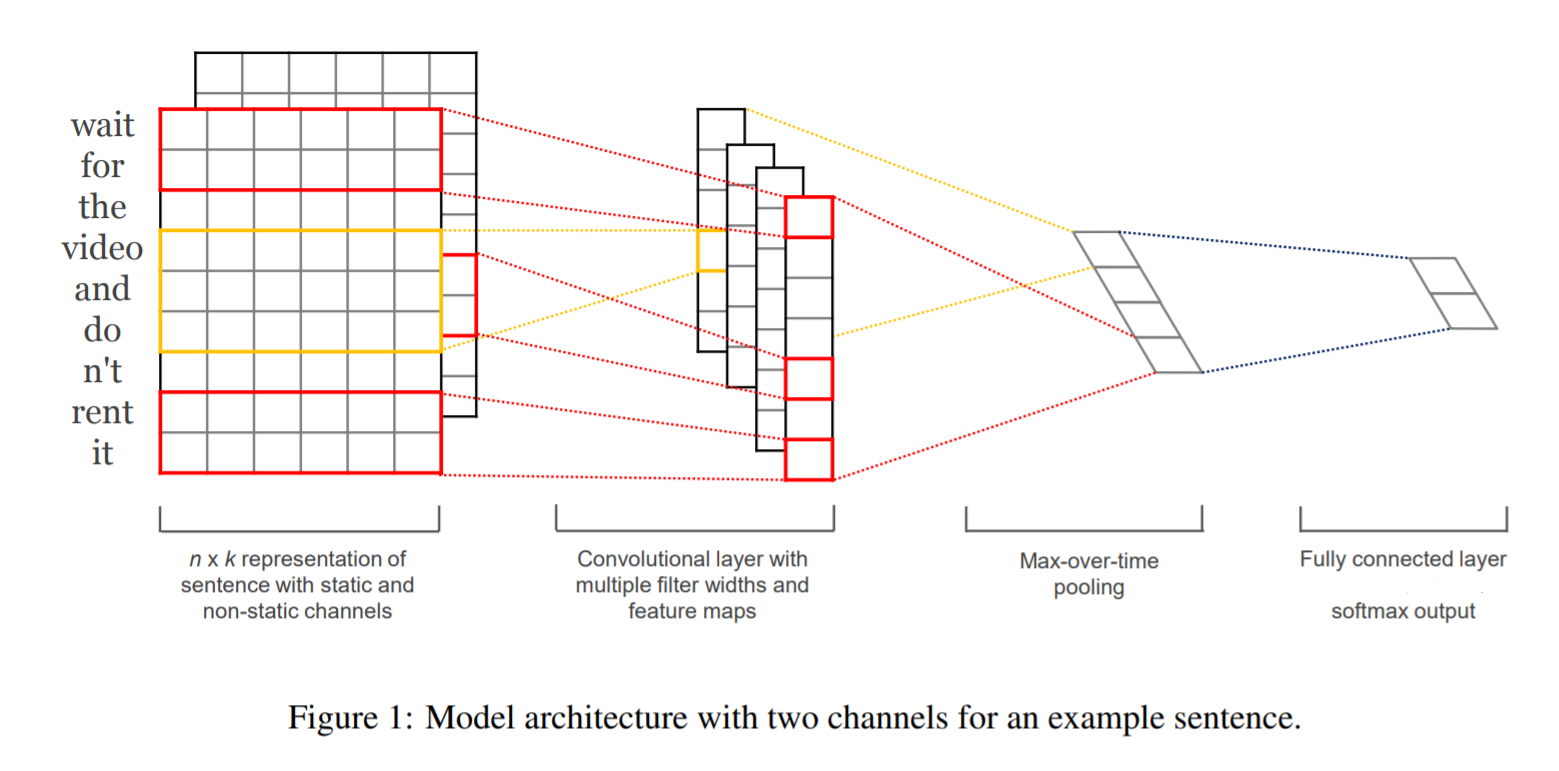
\includegraphics[width=0.5\textwidth]{Diagram.png}
\end{figure}

\subsection{Training Details}
As with the RNN, I implemented this model in PyTorch. I used 300 dimensional pre-trained GloVe embeddings to transform input sentences. I used 3 different convolutional layers $(h=3,4,5)$, each with a depth of 20. I used the Adam optimizer with a learning rate of $lr=0.001.$ The model was trained with a batch size of 50 over 100 epochs.

\section{Experimental Results and Evaluation}
As mentioned earlier, the data was divided into roughly 70\% training data and 30\% testing data. I evaluated my models by seeing how often they could correctly guess the candidate when given an unlabeled paragraph from the testing set. In order to better understand my models' performance, I created two further "Baseline" models. The first Baseline model is the Linear Baseline, which returned a random guess over a linear distribution over the number of data points / candidate. The second Baseline model is the Softmax Baseline, which returned a random guess over the number of data points / candidate after being passed through a Softmax function in order to account for some candidates having more data than others.

The results of my experiments are summarized in the table below.

\begin{table}[htb]
 \caption{Results}
  \centering
  \begin{tabular}{ll}
    \toprule
    \cmidrule(r){1-2}
    Model     & \% Correct of Testing Data   \\
    \midrule
    RNN + Classifier & 47.347\% (705/1489)\\
    CNN + Classifier & 33.311\% (496/1489) \\
    Softmax Baseline & 22.633\% (337/1489)\\
    Linear Baseline & 10.208\% (152/1489)
    \bottomrule
  \end{tabular}
\end{table}

The RNN was clearly the strongest performer, followed by the CNN and then the two Baseline models. It's encouraging to see that both models performed better than just the baseline, but neither model performed outstandingly.

I believe the RNN was the strongest performer because it was more apt to the task. The use of a GRU was very important, especially as some of the input sequences were up to 396 words in length! It was important that the GRU was able to remember and use context from the entire input sequence.

I believe the CNN did not perform as well due to its limited scope in words. As implemented in the paper, the network takes the most important $h-$word phrase at each time step. Due to the extreme length of some inputs, it is likely that the CNN could not keep attention for long enough. Some possible solutions to this problem could be to add more convolutions while keeping more than just the max element during the pooling step. Another possible solution is to consider something like a transformer architecture where a linear combination of all word vectors in a phrase are sent to the next layer at each time step rather than many local linear combinations.

\subsection{Discussion of Error}
I believe that this relatively poor performance is due to the relatively poor data. Because there was no large, publicly available data set for this project, I had to create my own. Some of the data comes from automatic YouTube transcriptions, meaning that I lose a lot of data including punctuation, and I lose accuracy, as the transcription algorithms are not always correct. This combined with the relatively small amount of data that I was able to collect likely is partially responsible for the error seen.

\section{Conclusion}
In this paper, I developed two neural networks in order to classify sequences of words. Though neither model excelled, both performed better than the baseline. I determined that for this task, an RNN was a better model for the CNN and suggested some possible changes to the CNN architecture that could perhaps improve performance.

\bibliographystyle{unsrt}  
%\bibliography{references}  %%% Remove comment to use the external .bib file (using bibtex).
%%% and comment out the ``thebibliography'' section.


%%% Comment out this section when you \bibliography{references} is enabled.
\begin{thebibliography}{1}

\bibitem{githubdataset}
2020 Presidential Candidate Dataset
\newblock \url{https://github.com/doshiro/2020-presidential-candidate-dataset} 

\bibitem{nnprimer}
\newblock Yoav Goldberg. 2016. A primer on neural network
models for natural language processing. J. Artif. Intell. Res., 57:345–420.

\bibitem{cnnpaper}
Kim, Yoon. 2014. Convolutional Neural Networks for Sentence Classification. arXiv:1408.5882 [cs.CL]

\bibitem{GRU}
Mani, Kaushik. 2019. GRU's and LSTM's. \url{https://towardsdatascience.com/grus-and-lstm-s-741709a9b9b1}

\end{thebibliography}


\end{document}
